
\documentclass[letterpaper,12pt]{article}

\usepackage[authoryear]{natbib}
\usepackage{url}
\usepackage{graphicx}

\title{Details about the spoked wheel dendrograms for the Fish and Fisheries manuscript}

\author{Daniel Ricard \textit{et al.}}

\begin{document}
\maketitle
\section{Introduction}
We are interested in determining the taxonomic bias of 1) fish species
that are caught commercially and 2) those that undergo formal stock
assessments. The accepted taxonomic coverage of fish species is
provided by FishBase. The commercial catch data available from the Sea
Around Us Project (SAUP) provides the reference for the taxonomic
coverage of harvested species. The RAM Legacy database contains
timeseries data for harvested species that undergo proper stock
assessments.

Establishing the taxonomic biases of the catch and assessment data
requires us to identify a common denominator between the three data
sources. Large Marine Ecosystems (LMEs) provide a geographical zoning
system that can be used to identify where different fish species occur
in the world's oceans. However, LMEs were designed to identify shallow
and coastal regions of the oceans and do not encompass open ocean
regions.  Highly migratory species that do not predominantly inhabit
coastal habitats need to be treated separetely.

Central to the RAM Legacy database is the concept of a
population/stock. A stock links a species to an oceanic region under
consideration for a stock assessment. A given fish species can have multiple
stocks.

The RAM Legacy database and SAUP also contain non-fish species which
should be removed from the comparison with FishBase. Similarly,
species that are highly migratory should also be removed from the comparison. 

A species list is generated for each of the three datasets. For each
species in the list, the number of different LMEs that species
appears is recorded. 

\section{Taxonomic coverage}


The FishBase taxonomic coverage can be found on Figure~\ref{fig:fishbase}.


The SAUP taxonomic coverage can be found on Figure~\ref{fig:SAUP}.


The srdb taxonomic coverage can be found on Figure~\ref{fig:srdb}.



\begin{figure}\label{fig:fishbase}
\begin{center}
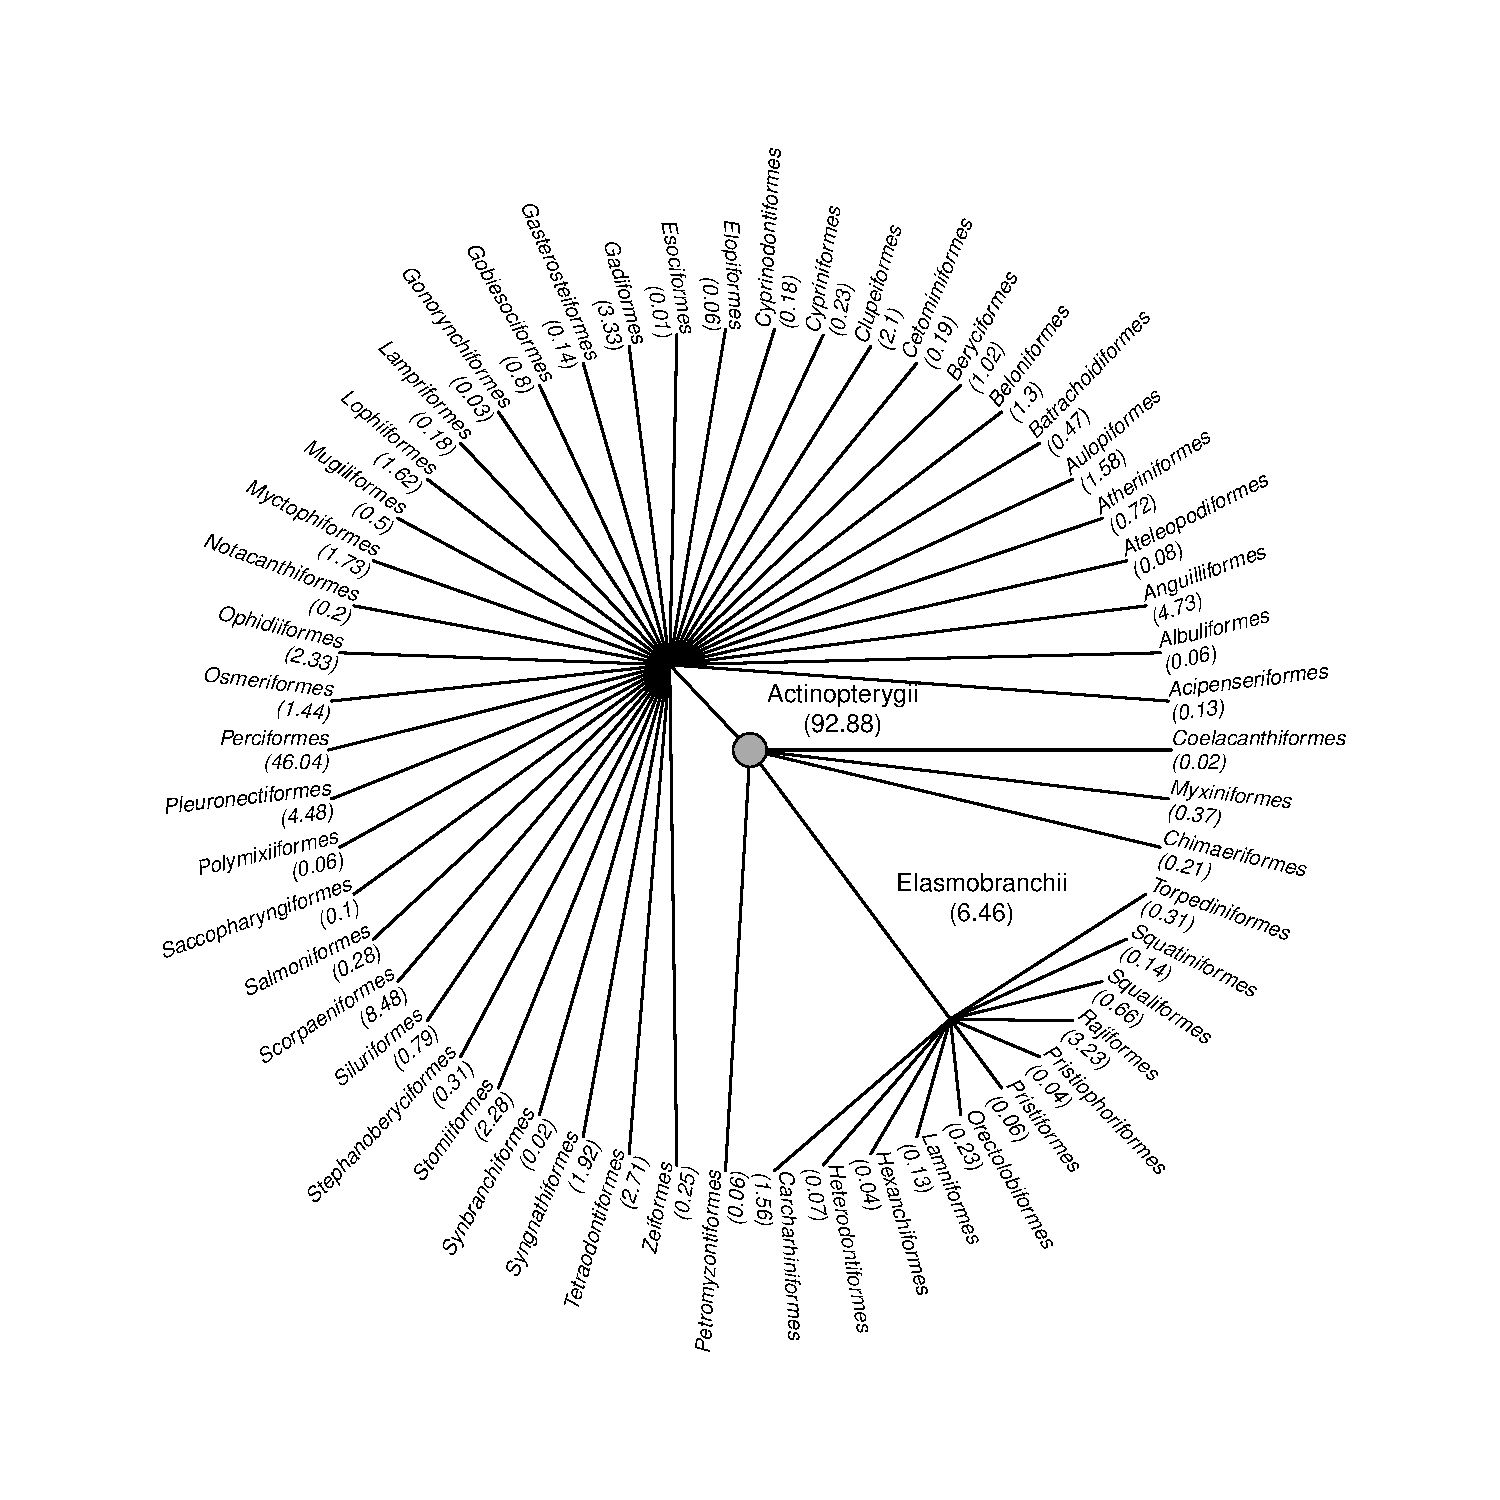
\includegraphics[width=15cm]{/home/srdbadmin/SQLpg/srdb/trunk/projects/fishandfisheries/R/FishBase-byorder.pdf}
\end{center}
\caption{FishBase}
\end{figure}


\begin{figure}\label{fig:SAUP}
\begin{center}
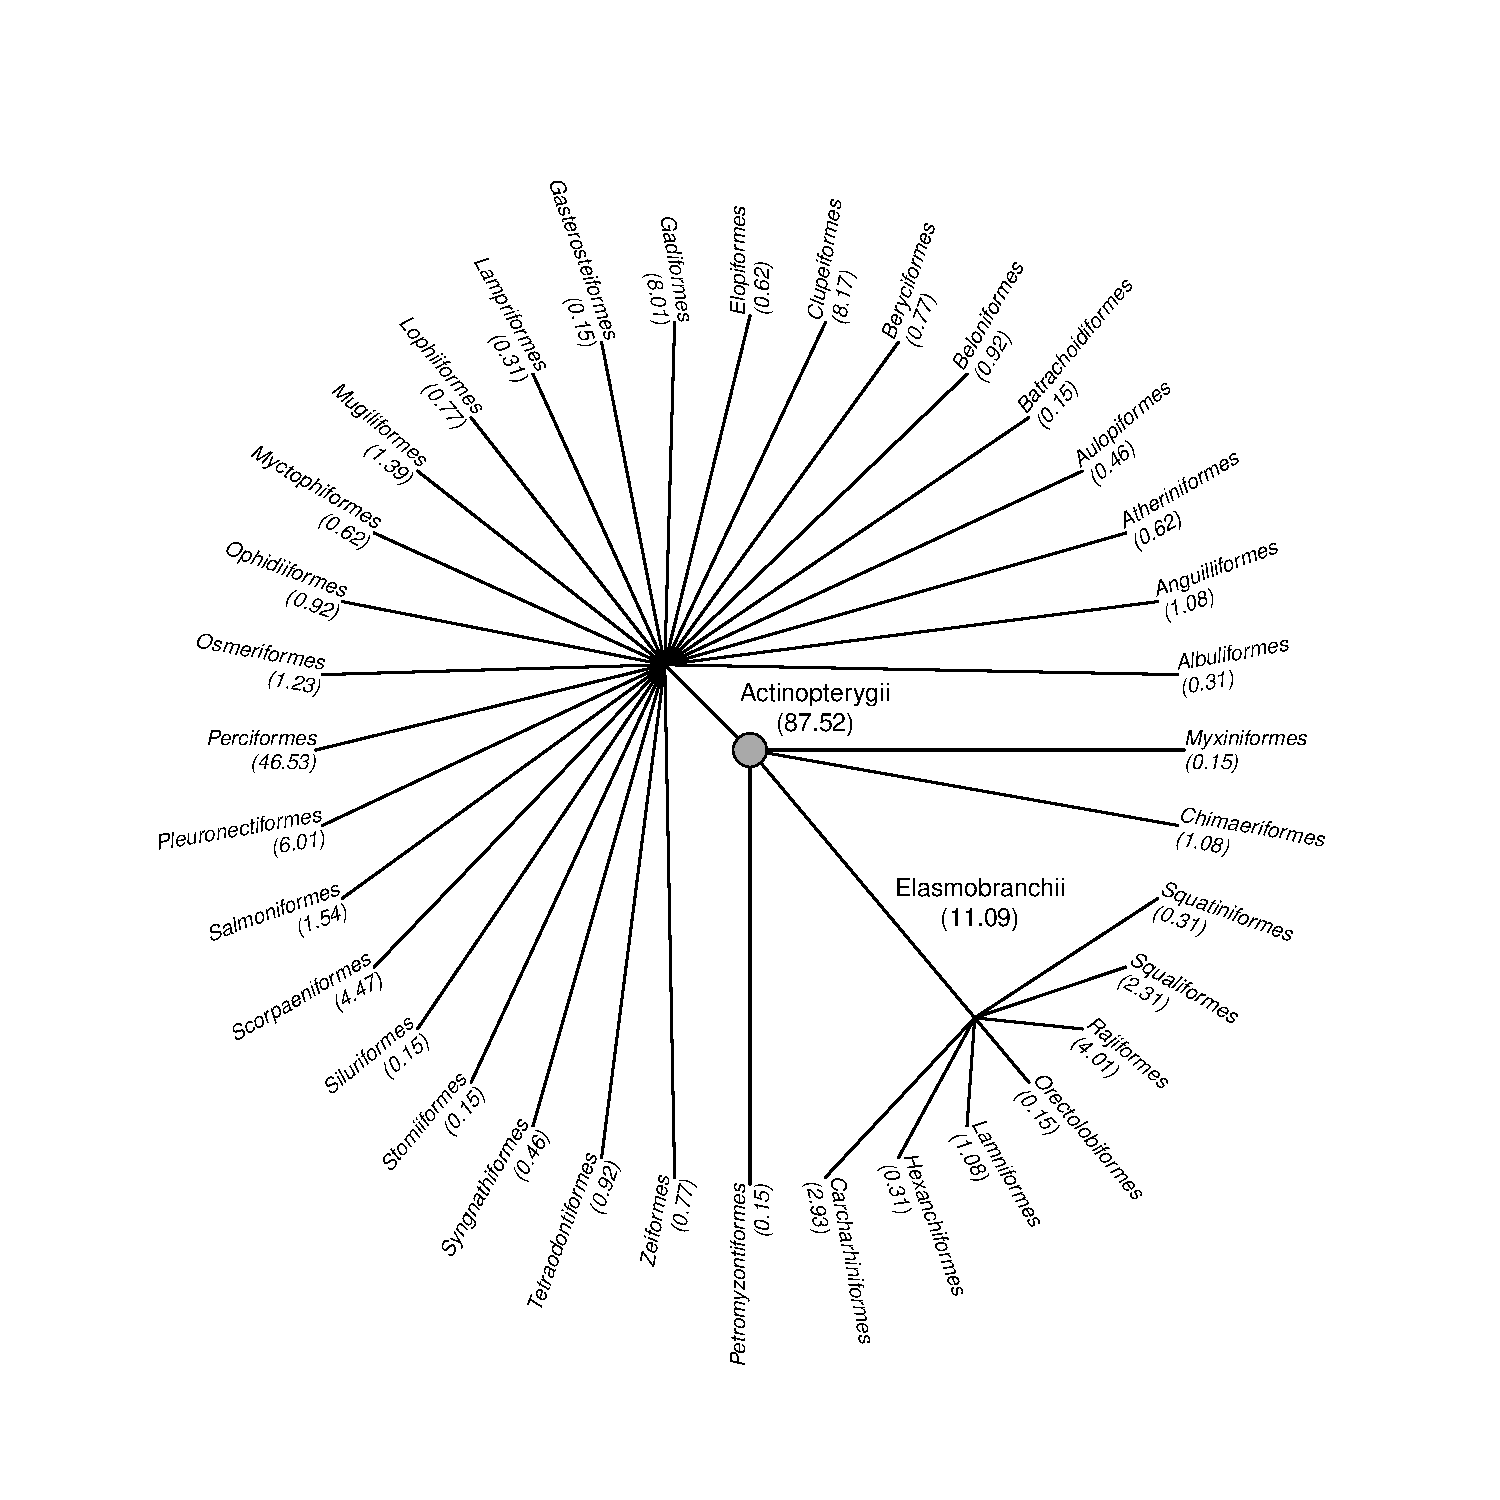
\includegraphics[width=15cm]{/home/srdbadmin/SQLpg/srdb/trunk/projects/fishandfisheries/R/SAUP-byorder.pdf}
\end{center}
\caption{SAUP - simulated as a sample from FishBase}
\end{figure}

\begin{figure}\label{fig:srdb}
\begin{center}
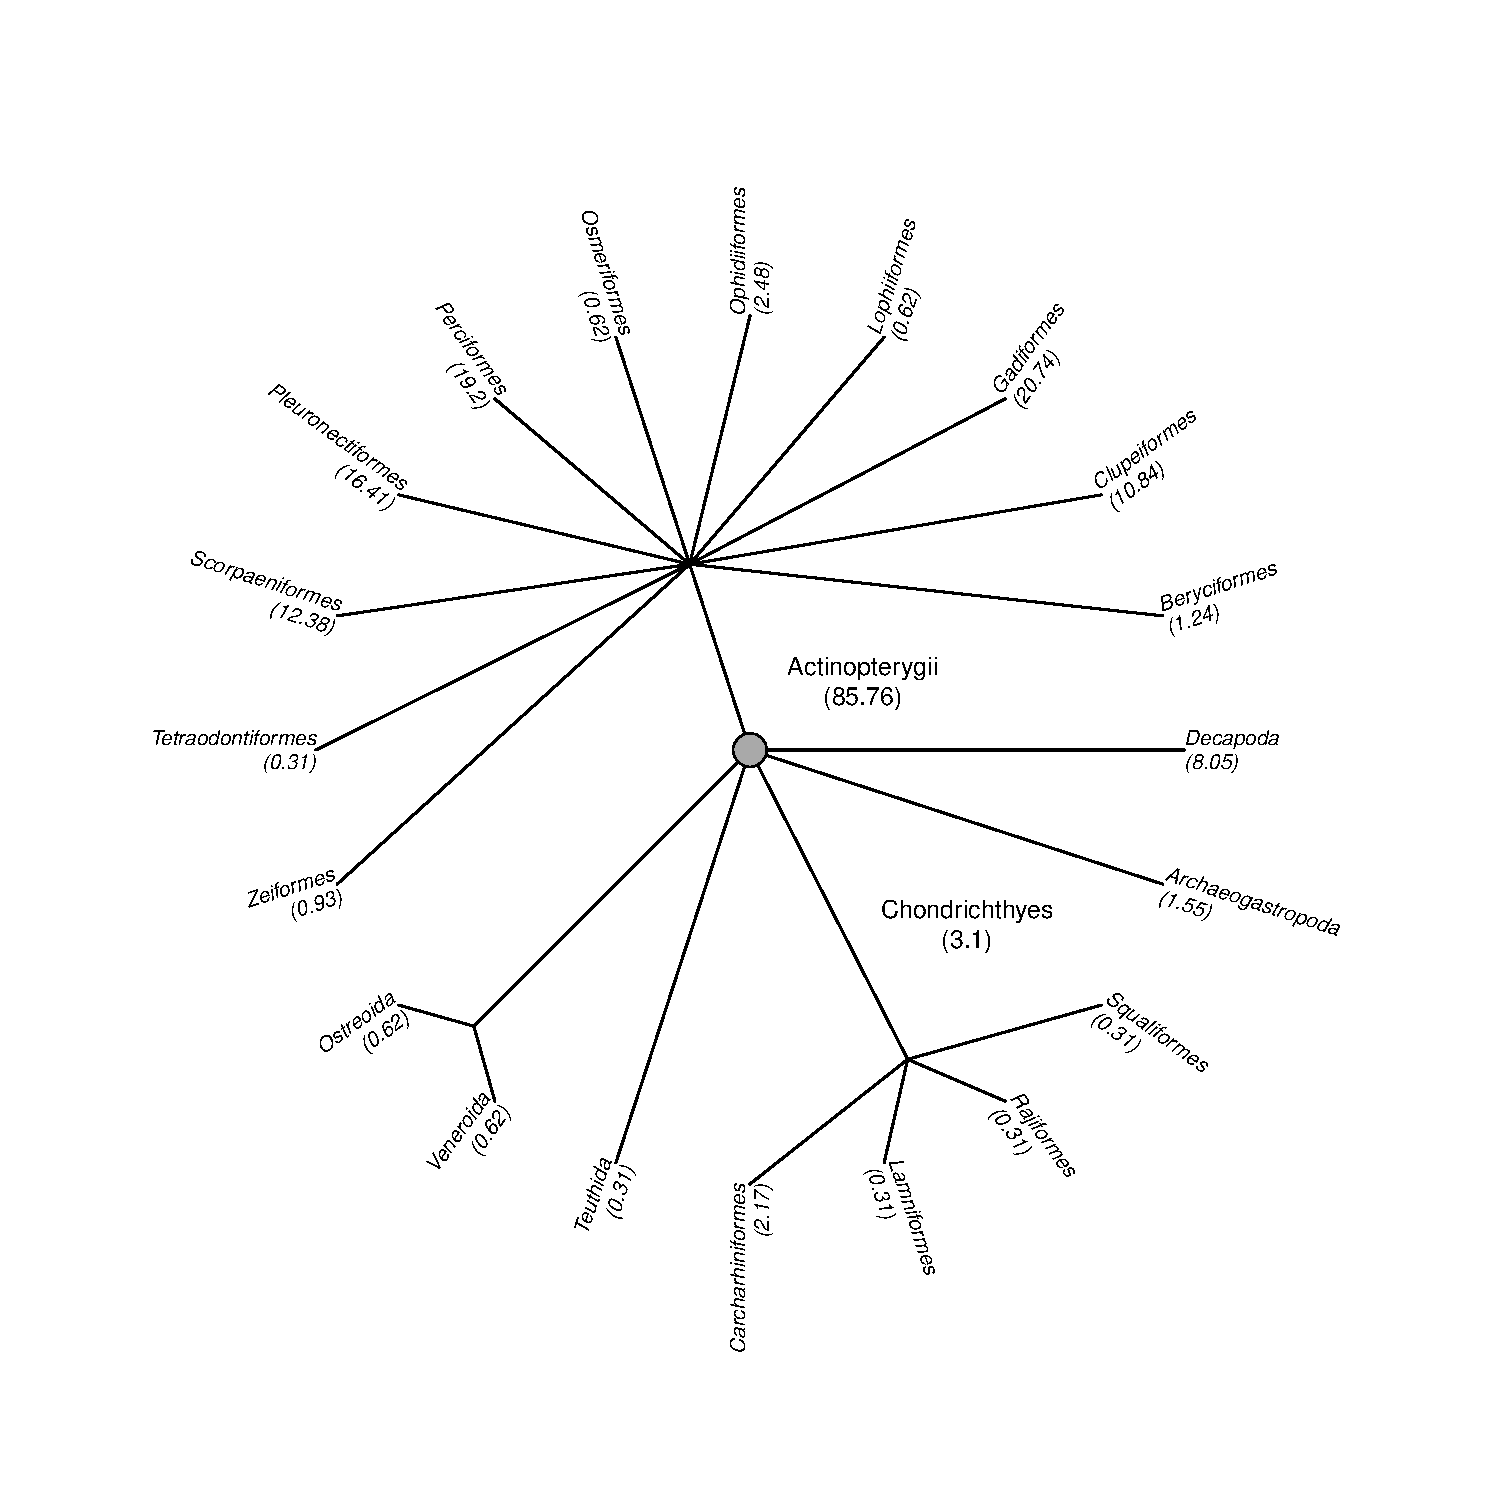
\includegraphics[width=15cm]{/home/srdbadmin/SQLpg/srdb/trunk/projects/fishandfisheries/R/srdb-byorder.pdf}
\end{center}
\caption{srdb}
\end{figure}


\section{Taxonomic bias}

To examine the taxonomic bias of the SAUP data and that of the RAM
Legacy database, the FishBase spoked wheel dendrogram is used as the
accepted taxonomic coverage for fish species (top-left panel of
Figure~\ref{fig:4panel}). The dendrogram is generated for the SAUP
dataset while maintaining the FishBase branching pattern (top-right
panel of Figure~\ref{fig:4panel}). The same is done to compare the RAM
Legacy database to the SAUP dataset (bottom panel of
Figure~\ref{fig:4panel})


\begin{figure}
\begin{center}
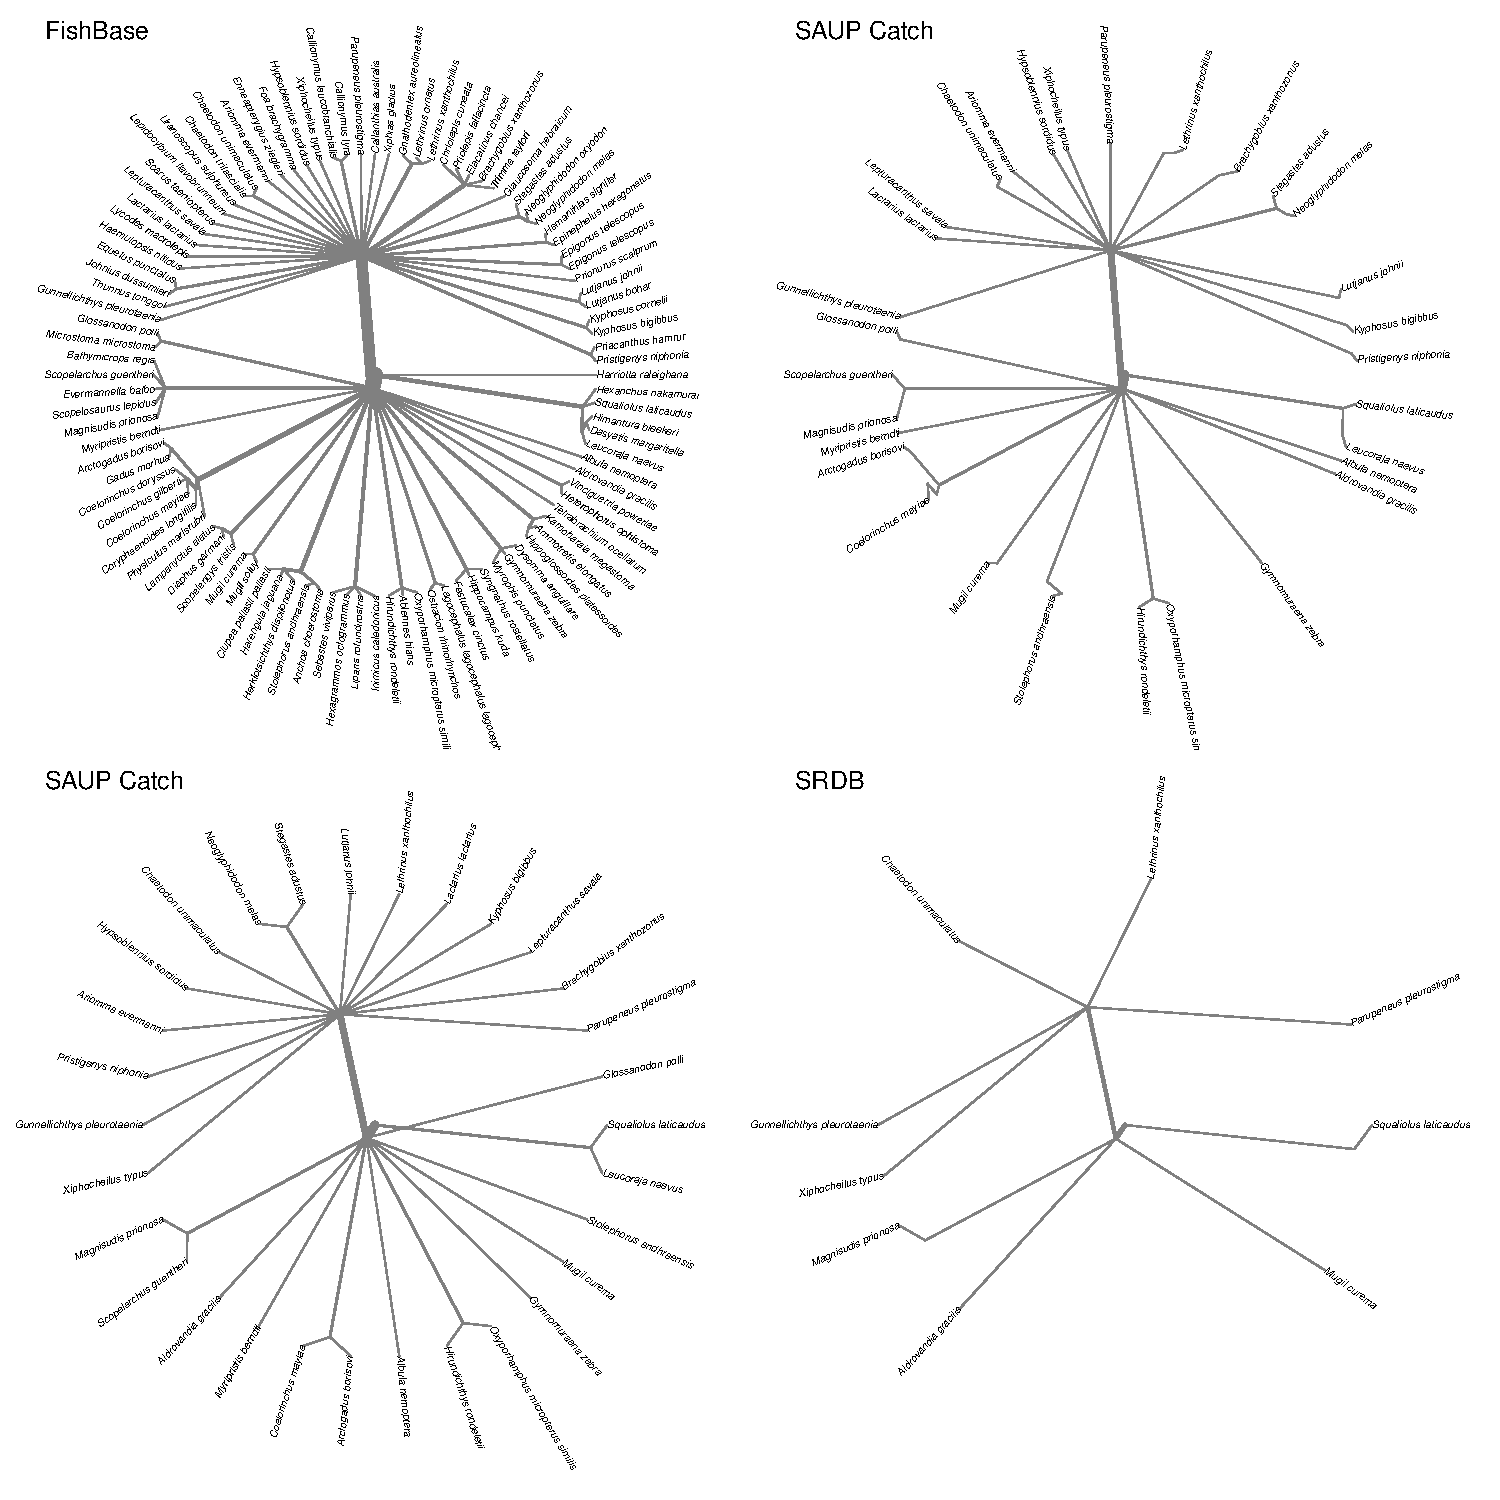
\includegraphics[width=15cm]{/home/srdbadmin/SQLpg/srdb/trunk/projects/fishandfisheries/R/fourpanel-byorder.pdf}
\end{center}
\caption{SAUP compared to FishBase and srdb compared to SAUP}
\end{figure}\label{fig:4panel}

\end{document}

